\documentclass[11pt]{article}
\usepackage[margin=1.6cm]{geometry}
\usepackage[T1]{fontenc}
\usepackage[utf8]{inputenc}
\usepackage{tikz}
\usetikzlibrary{arrows.meta,positioning}
\usepackage{xcolor}
\usepackage{hyperref}
\definecolor{ink}{HTML}{243246}
\definecolor{teal}{HTML}{DBEFE9}
\definecolor{rose}{HTML}{F6DFE2}
\definecolor{gold}{HTML}{F8EDCF}
\pagestyle{plain}
\setlength{\parindent}{0pt}
\tikzset{box/.style={draw=ink,rounded corners=4pt,fill=teal,align=center,text width=6.2cm,minimum height=.9cm,font=\small},arr/.style={-{Stealth},draw=ink,thick}}
\begin{document}
\begin{center}{\LARGE\bfseries The Light We Leave On}\\[5pt]{\large Playable story map}\end{center}
Four adult women. Free conversation. Independent relationships and a shared summer. This map is generated from the playable story catalog; edges are scene transitions, not dialogue options.
\vspace{8pt}\begin{center}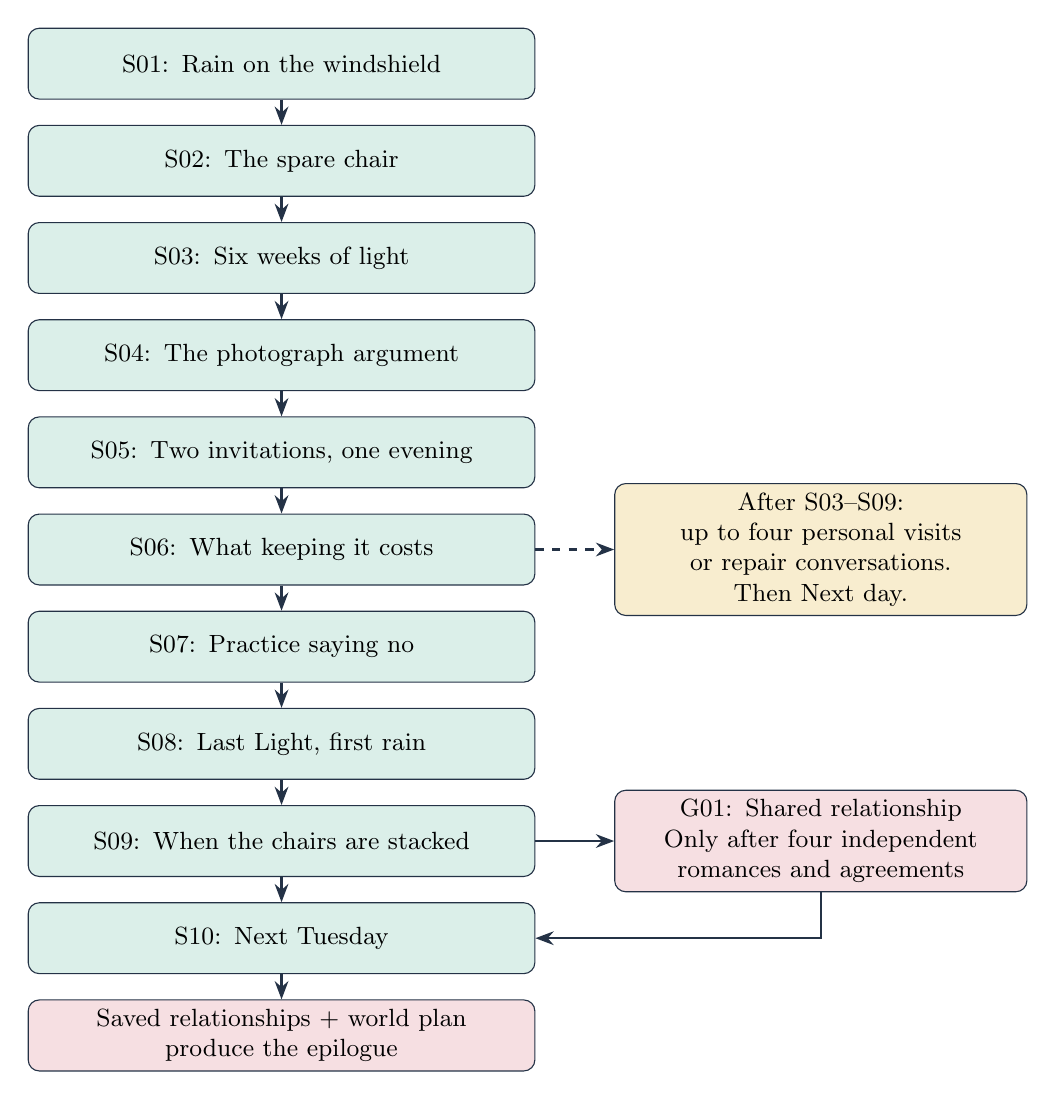
\begin{tikzpicture}[node distance=.32cm]
\node[box] (S01) {S01: Rain on the windshield};
\node[box,below=of S01] (S02) {S02: The spare chair};
\draw[arr] (S01) -- (S02);
\node[box,below=of S02] (S03) {S03: Six weeks of light};
\draw[arr] (S02) -- (S03);
\node[box,below=of S03] (S04) {S04: The photograph argument};
\draw[arr] (S03) -- (S04);
\node[box,below=of S04] (S05) {S05: Two invitations, one evening};
\draw[arr] (S04) -- (S05);
\node[box,below=of S05] (S06) {S06: What keeping it costs};
\draw[arr] (S05) -- (S06);
\node[box,below=of S06] (S07) {S07: Practice saying no};
\draw[arr] (S06) -- (S07);
\node[box,below=of S07] (S08) {S08: Last Light, first rain};
\draw[arr] (S07) -- (S08);
\node[box,below=of S08] (S09) {S09: When the chairs are stacked};
\draw[arr] (S08) -- (S09);
\node[box,below=of S09] (S10) {S10: Next Tuesday};
\draw[arr] (S09) -- (S10);
\node[box,fill=gold,right=1cm of S06,text width=5cm] (visits) {After S03--S09:\\up to four personal visits\\or repair conversations.\\Then Next day.};
\draw[arr,dashed] (S06.east) -- (visits.west);
\node[box,fill=rose,right=1cm of S09,text width=5cm] (group) {G01: Shared relationship\\Only after four independent\\romances and agreements};
\draw[arr] (S09.east) -- (group.west);\draw[arr] (group.south) |- (S10.east);
\node[box,fill=rose,below=of S10] (end) {Saved relationships + world plan\\produce the epilogue};
\draw[arr] (S10) -- (end);
\end{tikzpicture}\end{center}
\textbf{Not a single romance track.} Shared scenes advance the calendar; personal chapters advance only when visited. A skipped visit never invents a date or a broken promise.
\newpage
\section*{How a conversation becomes a branch}
\begin{center}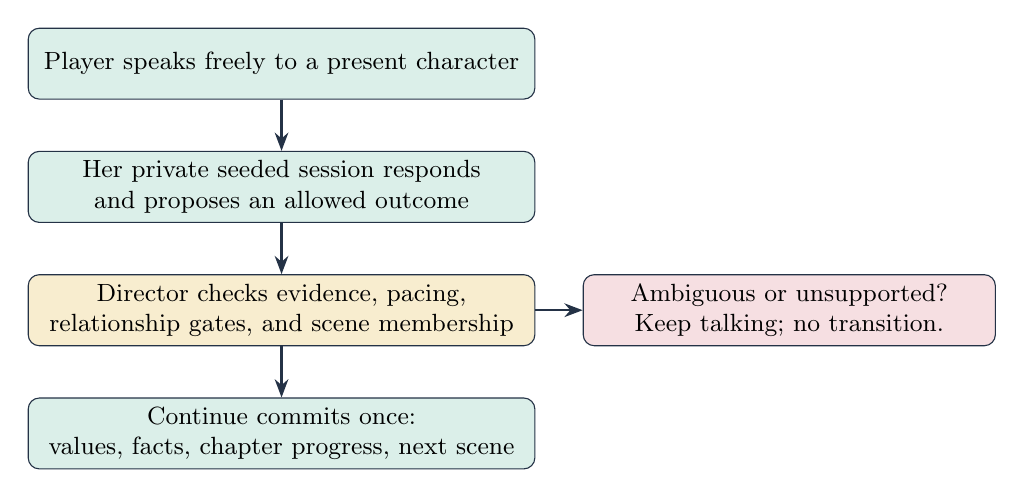
\begin{tikzpicture}[node distance=.65cm]
\node[box] (talk) {Player speaks freely to a present character};
\node[box,below=of talk] (model) {Her private seeded session responds\\and proposes an allowed outcome};
\node[box,fill=gold,below=of model] (guard) {Director checks evidence, pacing,\\relationship gates, and scene membership};
\node[box,below=of guard] (commit) {Continue commits once:\\values, facts, chapter progress, next scene};
\node[box,fill=rose,right=.6cm of guard,text width=5cm] (stay) {Ambiguous or unsupported?\\Keep talking; no transition.};
\draw[arr] (talk)--(model);\draw[arr] (model)--(guard);\draw[arr] (guard)--(commit);\draw[arr] (guard)--(stay);
\end{tikzpicture}\end{center}
\subsection*{Possible outcomes inside every personal chapter}
\begin{itemize}\item Connect: trust and ease; not automatically attraction.\item Romance: explicit mutual interest, kisses, cuddles, and dates; commitment in chapter 6.\item Together: each woman independently opts into the shared relationship in chapter 6; G01 settles the group agreement.\item Friendship: optional when romance is declined.\item Uncertainty: space to decide.\item Hurt: a named boundary and private repair.\item Leave: end the visit without inventing consent.\end{itemize}
\subsection*{Repair detour}
A specific apology and reciprocal agreement reopen the path. Space keeps it paused. Repeated pressure after a warning or an explicit ending closes it. No apology forces forgiveness.
\subsection*{Shared intersections}
\begin{itemize}\item S04: publicity versus privacy; Hana, Mira, and Leila disagree.\item S05: overlapping invitations; communicate rather than silently double-book.\item S06: a sustainable smaller caf\'e or a supper club; independent ambitions remain real.\item S07: defend reasonable boundaries or blame a convenient person.\item S08: adapt Last Light to rain; a small gathering still matters.\end{itemize}
\newpage
\section*{Hana, 24}
Observant, quietly stubborn café shift lead and illustrator. Gentle precise humor. Names broken appliances. Helps too readily and must learn to ask before helping.
\medskip
\textbf{Wants:} Be wanted for her company, not only her care. Explore illustration as well as the café.
\medskip
\begin{center}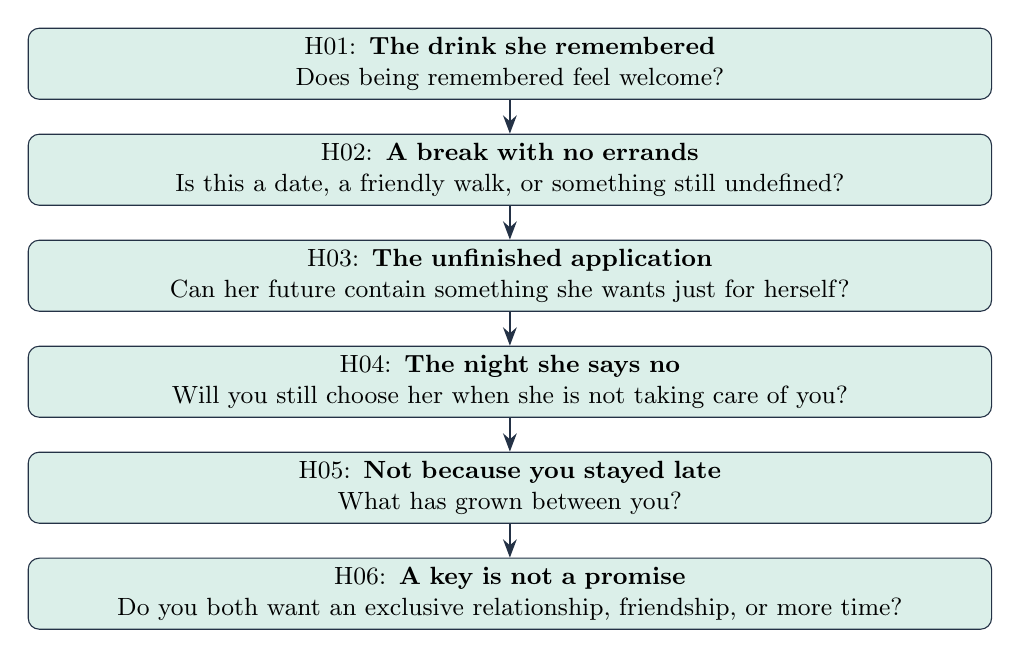
\begin{tikzpicture}[node distance=.43cm]
\node[box,text width=12cm] (H01) {H01: \textbf{The drink she remembered}\\ Does being remembered feel welcome?};
\node[box,text width=12cm,below=of H01] (H02) {H02: \textbf{A break with no errands}\\ Is this a date, a friendly walk, or something still undefined?};
\draw[arr] (H01) -- (H02);
\node[box,text width=12cm,below=of H02] (H03) {H03: \textbf{The unfinished application}\\ Can her future contain something she wants just for herself?};
\draw[arr] (H02) -- (H03);
\node[box,text width=12cm,below=of H03] (H04) {H04: \textbf{The night she says no}\\ Will you still choose her when she is not taking care of you?};
\draw[arr] (H03) -- (H04);
\node[box,text width=12cm,below=of H04] (H05) {H05: \textbf{Not because you stayed late}\\ What has grown between you?};
\draw[arr] (H04) -- (H05);
\node[box,text width=12cm,below=of H05] (H06) {H06: \textbf{A key is not a promise}\\ Do you both want an exclusive relationship, friendship, or more time?};
\draw[arr] (H05) -- (H06);
\end{tikzpicture}\end{center}
\textbf{Schedule:} Chapters 1--6 unlock after S03, S04, S05, S06, S08, and S09 respectively. They may be visited later in order.
\medskip
\textbf{Branching at each box:} connect / romance / friend / uncertain / hurt / leave. Hurt offers the repair detour before further romance. Every normal completion returns to the visit window.
\medskip
\textbf{Romantic progression:} chapter 2 invites hand-holding or leaning close; chapter 5 offers a first kiss; chapter 6 includes a kiss, cuddle, or farewell embrace. Touch remains optional and mutual.
\medskip
\textbf{Final branches:} exclusive partner; explicit consent to the all-four relationship; continuing dates; optional friendship; or distance. Four independent shared consents unlock G01. The world ending is independent.
\newpage
\section*{Mira, 25}
Playful bicycle mechanic and cinema projectionist. Brave about small things, evasive about vulnerability. Repairs things carefully and describes doing so recklessly.
\medskip
\textbf{Wants:} Be enjoyed when quiet, not only when entertaining. Begin a technical certification course.
\medskip
\begin{center}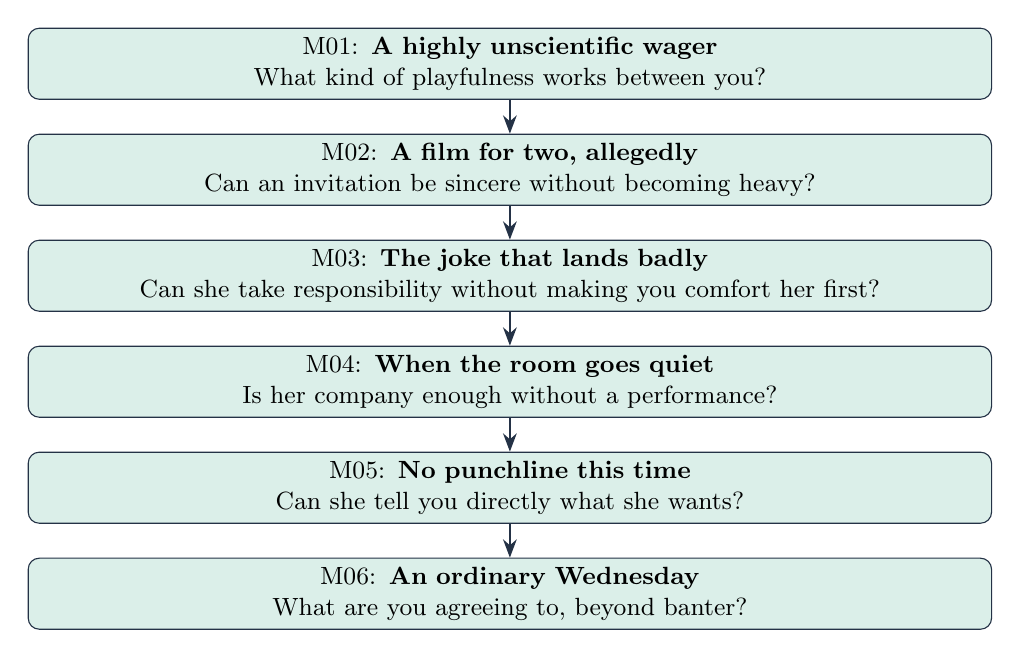
\begin{tikzpicture}[node distance=.43cm]
\node[box,text width=12cm] (M01) {M01: \textbf{A highly unscientific wager}\\ What kind of playfulness works between you?};
\node[box,text width=12cm,below=of M01] (M02) {M02: \textbf{A film for two, allegedly}\\ Can an invitation be sincere without becoming heavy?};
\draw[arr] (M01) -- (M02);
\node[box,text width=12cm,below=of M02] (M03) {M03: \textbf{The joke that lands badly}\\ Can she take responsibility without making you comfort her first?};
\draw[arr] (M02) -- (M03);
\node[box,text width=12cm,below=of M03] (M04) {M04: \textbf{When the room goes quiet}\\ Is her company enough without a performance?};
\draw[arr] (M03) -- (M04);
\node[box,text width=12cm,below=of M04] (M05) {M05: \textbf{No punchline this time}\\ Can she tell you directly what she wants?};
\draw[arr] (M04) -- (M05);
\node[box,text width=12cm,below=of M05] (M06) {M06: \textbf{An ordinary Wednesday}\\ What are you agreeing to, beyond banter?};
\draw[arr] (M05) -- (M06);
\end{tikzpicture}\end{center}
\textbf{Schedule:} Chapters 1--6 unlock after S03, S04, S05, S06, S08, and S09 respectively. They may be visited later in order.
\medskip
\textbf{Branching at each box:} connect / romance / friend / uncertain / hurt / leave. Hurt offers the repair detour before further romance. Every normal completion returns to the visit window.
\medskip
\textbf{Romantic progression:} chapter 2 invites hand-holding or leaning close; chapter 5 offers a first kiss; chapter 6 includes a kiss, cuddle, or farewell embrace. Touch remains optional and mutual.
\medskip
\textbf{Final branches:} exclusive partner; explicit consent to the all-four relationship; continuing dates; optional friendship; or distance. Four independent shared consents unlock G01. The world ending is independent.
\newpage
\section*{Leila, 26}
Thoughtful freelance photographer with dry humor. Comfortable with silence; sometimes uses it to avoid answers. Wants to participate rather than always observe.
\medskip
\textbf{Wants:} Intimacy compatible with independence and a photography residency.
\medskip
\begin{center}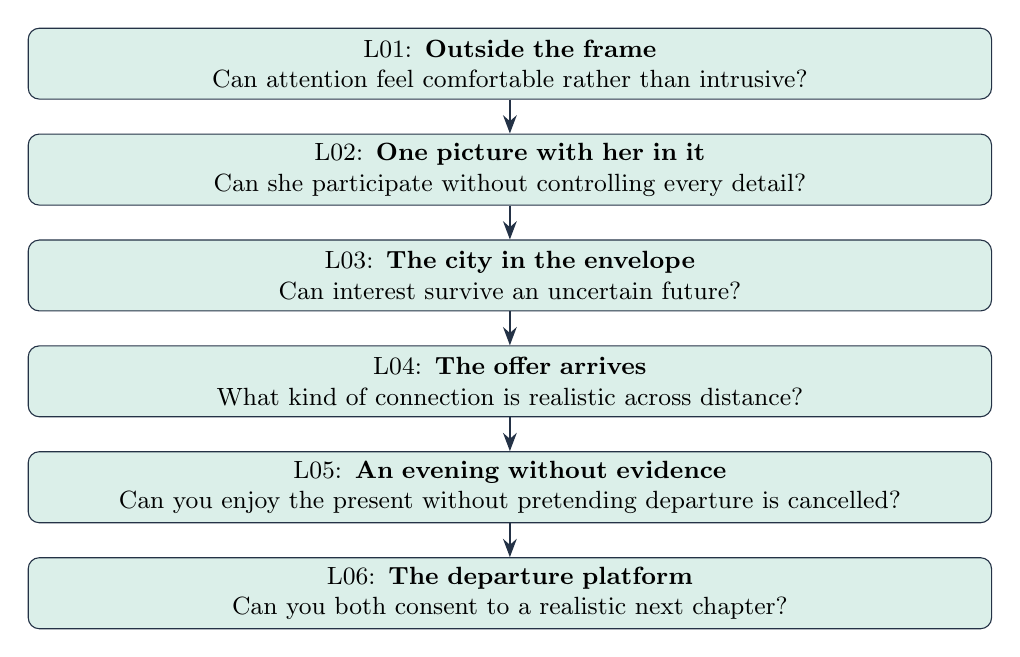
\begin{tikzpicture}[node distance=.43cm]
\node[box,text width=12cm] (L01) {L01: \textbf{Outside the frame}\\ Can attention feel comfortable rather than intrusive?};
\node[box,text width=12cm,below=of L01] (L02) {L02: \textbf{One picture with her in it}\\ Can she participate without controlling every detail?};
\draw[arr] (L01) -- (L02);
\node[box,text width=12cm,below=of L02] (L03) {L03: \textbf{The city in the envelope}\\ Can interest survive an uncertain future?};
\draw[arr] (L02) -- (L03);
\node[box,text width=12cm,below=of L03] (L04) {L04: \textbf{The offer arrives}\\ What kind of connection is realistic across distance?};
\draw[arr] (L03) -- (L04);
\node[box,text width=12cm,below=of L04] (L05) {L05: \textbf{An evening without evidence}\\ Can you enjoy the present without pretending departure is cancelled?};
\draw[arr] (L04) -- (L05);
\node[box,text width=12cm,below=of L05] (L06) {L06: \textbf{The departure platform}\\ Can you both consent to a realistic next chapter?};
\draw[arr] (L05) -- (L06);
\end{tikzpicture}\end{center}
\textbf{Schedule:} Chapters 1--6 unlock after S03, S04, S05, S06, S08, and S09 respectively. They may be visited later in order.
\medskip
\textbf{Branching at each box:} connect / romance / friend / uncertain / hurt / leave. Hurt offers the repair detour before further romance. Every normal completion returns to the visit window.
\medskip
\textbf{Romantic progression:} chapter 2 invites hand-holding or leaning close; chapter 5 offers a first kiss; chapter 6 includes a kiss, cuddle, or farewell embrace. Touch remains optional and mutual.
\medskip
\textbf{Final branches:} exclusive partner; explicit consent to the all-four relationship; continuing dates; optional friendship; or distance. Four independent shared consents unlock G01. The world ending is independent.
\newpage
\section*{Tessa, 27}
Warm carpenter and theater stagehand. Patient, grounded, quietly playful. Calls inconveniences fine until resentful; must name her needs. Bakes handsome but questionable bread.
\medskip
\textbf{Wants:} Be invited when nothing needs fixing. Take recurring paid theater work.
\medskip
\begin{center}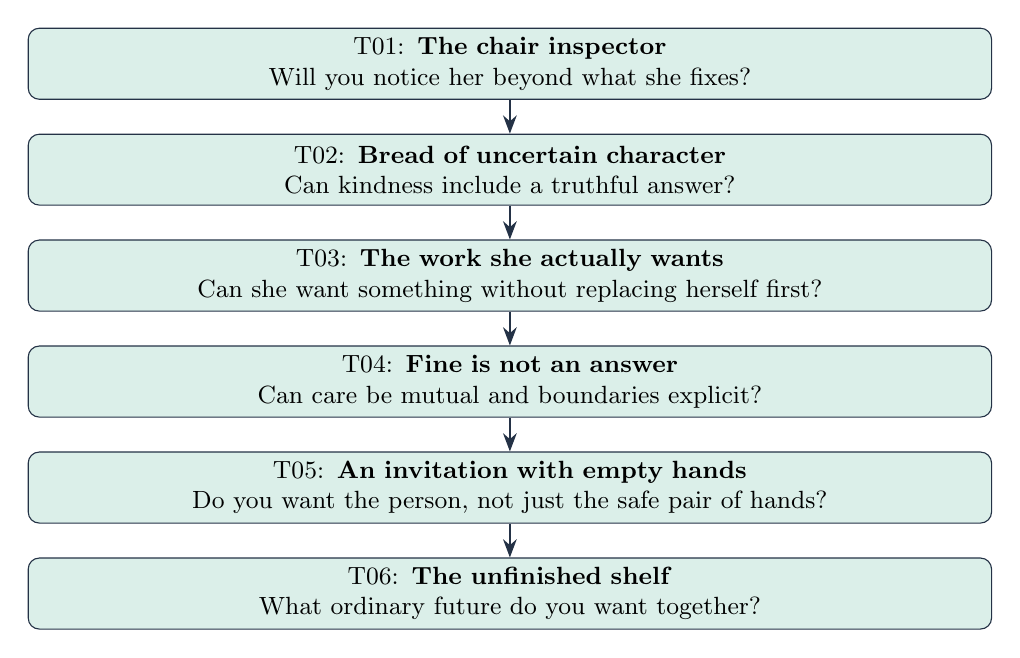
\begin{tikzpicture}[node distance=.43cm]
\node[box,text width=12cm] (T01) {T01: \textbf{The chair inspector}\\ Will you notice her beyond what she fixes?};
\node[box,text width=12cm,below=of T01] (T02) {T02: \textbf{Bread of uncertain character}\\ Can kindness include a truthful answer?};
\draw[arr] (T01) -- (T02);
\node[box,text width=12cm,below=of T02] (T03) {T03: \textbf{The work she actually wants}\\ Can she want something without replacing herself first?};
\draw[arr] (T02) -- (T03);
\node[box,text width=12cm,below=of T03] (T04) {T04: \textbf{Fine is not an answer}\\ Can care be mutual and boundaries explicit?};
\draw[arr] (T03) -- (T04);
\node[box,text width=12cm,below=of T04] (T05) {T05: \textbf{An invitation with empty hands}\\ Do you want the person, not just the safe pair of hands?};
\draw[arr] (T04) -- (T05);
\node[box,text width=12cm,below=of T05] (T06) {T06: \textbf{The unfinished shelf}\\ What ordinary future do you want together?};
\draw[arr] (T05) -- (T06);
\end{tikzpicture}\end{center}
\textbf{Schedule:} Chapters 1--6 unlock after S03, S04, S05, S06, S08, and S09 respectively. They may be visited later in order.
\medskip
\textbf{Branching at each box:} connect / romance / friend / uncertain / hurt / leave. Hurt offers the repair detour before further romance. Every normal completion returns to the visit window.
\medskip
\textbf{Romantic progression:} chapter 2 invites hand-holding or leaning close; chapter 5 offers a first kiss; chapter 6 includes a kiss, cuddle, or farewell embrace. Touch remains optional and mutual.
\medskip
\textbf{Final branches:} exclusive partner; explicit consent to the all-four relationship; continuing dates; optional friendship; or distance. Four independent shared consents unlock G01. The world ending is independent.
\newpage
\section*{Endings and visual staging}
\begin{center}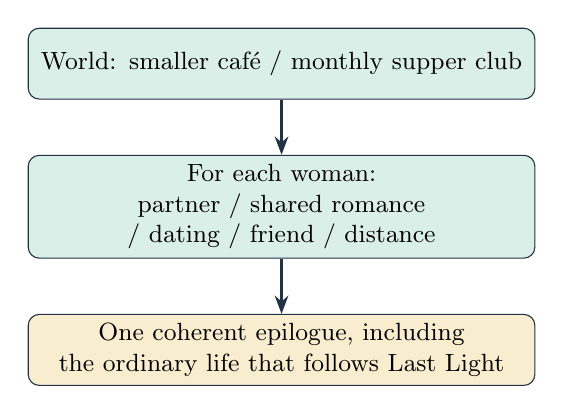
\begin{tikzpicture}[node distance=.7cm]
\node[box] (world) {World: smaller caf\'e / monthly supper club};
\node[box,below=of world] (rel) {For each woman:\\partner / shared romance / dating / friend / distance};
\node[box,fill=gold,below=of rel] (last) {One coherent epilogue, including\\the ordinary life that follows Last Light};
\draw[arr] (world)--(rel);\draw[arr] (rel)--(last);
\end{tikzpicture}\end{center}
\subsection*{Romantic payoffs}
\begin{itemize}\item Hana: breakfast between illustration deadlines.\item Mira: Wednesday dinners, with or without a joke.\item Leila: an imperfect first call and an affordable visit.\item Tessa: unfinished work can wait for chosen time together.\end{itemize}
\subsection*{Everyone ending: Enough Room for All of Us}
Four established romances, four private shared agreements, and G01 lead to an openly shared relationship. Individual dates, honest discussion of jealousy, long-distance inclusion, and personal space accompany a reunion of kisses, cuddles, and a very crowded sofa. Nobody consents on someone else's behalf.
\subsection*{Backgrounds}
Parked rainy car; warm café; narrow kitchen; sloping street; shared workshop; tiny cinema; lake railing; safe roof terrace; community hall; departure stop. Use reusable compositions with evening, rain, and event variants.
\subsection*{What is implemented}
35 authored scenes, a reusable private repair scene, saved relationship values, per-character inference sessions, native comic rendering, and individual or all-four romance endings. All four women have 12 illustrated poses and 120 skeletal motion variants each, with ten painted backgrounds. The interface includes a start menu, scene introductions, dialogue history, and autosave.
\subsection*{Reading the map}
Arrows show authored progression. They do not imply that every player visits every node. Full outcome rules are in SCENE\_GRAPH.md. Inference interprets intent probabilistically; guards do not guarantee perfect interpretation.
\end{document}
